\documentclass[a4paper,12pt]{article}
\usepackage[utf8]{inputenc}
\usepackage[croatian]{babel}
\usepackage[T1]{fontenc}
\usepackage{graphicx}
\usepackage{amsmath,amssymb,amsfonts,textcomp}
\usepackage{color}
\usepackage{calc}
\usepackage{url}
\usepackage{hyperref}
\hypersetup{colorlinks=true, linkcolor=black, filecolor=black, urlcolor=black, citecolor=black}
\usepackage{indentfirst}
\graphicspath{ {img/} }

\usepackage[nottoc, numbib, chapter]{tocbibind}
\usepackage[authoryear, round]{natbib}
\usepackage{titlesec}
\newcommand{\sectionbreak}{\clearpage}
\usepackage{booktabs}
\usepackage{mathpazo}
\usepackage{algorithm}
\usepackage{algorithmicx}
\usepackage{algpseudocode}

\pretolerance=150

\begin{document}

\begin{titlepage}
	\center
	
	\textsc{\Large SVEUČILIŠTE U ZAGREBU}\\
	\vspace{0.4cm}
	\textsc{\Large \textbf{FAKULTET ELEKTROTEHNIKE I RAČUNARSTVA}}
	\vspace{2.5cm}
	\vfill\vfill
    
	\textsc{\Large Projekt iz Bioinformatike}
	\vspace{0.5cm}
	
	{\huge\bfseries Računanje najduljeg zajedničkog prefiksa temeljeno na BWT}
	\vspace{1.2cm}
	
	\begin{minipage}{2.5\textwidth}
		\begin{flushleft}
			\large
			\textit{Autori}\\
			\textsc{Zvonimir Jurelinac, Tomislav Živec, Tonko Čupić}
		\end{flushleft}
	\end{minipage}

	\vspace{0.3cm}

	\begin{minipage}{2.5\textwidth}
		\begin{flushleft}
			\large
			\textit{Voditelj}\\
			doc.dr.sc \textsc{Mirjana Domazet- Lošo}
		\end{flushleft}
	\end{minipage}
	
	\vfill\vfill\vfill\vfill
	{\large Zagreb, prosinac 2017.}
		
\end{titlepage}

\newpage

\tableofcontents
\newpage

\section{Uvod}

Bioinformatika je grana znanosti koja usko povezuje biologiju i računarstvo, a ubrzano se razvijala zadnja dva desetljeća. Pojeftinjenje i sve veća dostupnost tehnologije sekvenciranja rezultirale su stvaranjem velikih skupova bioloških podataka. Često se kao zadatak u bioinformatici nameće analiza sekvence genoma. Pošto su te sekvence predugačke za uobičajenu pohranu i analizu, potrebno je za to koristiti posebne, prilagođene strukture podataka, kao što su sufiksna polja i polja najdužih zajedničkih prefiksa. 

Cilj projekta je bio čim učinkovitije implementirati algoritme 1 i 2 iz rada \cite{beller2013}, koristeći pritom gotovu knjižnicu za izgradnju sufiksnog polja, te potom ostvarenu implementaciju usporediti s originalnom, ali i s rezultatima prošlogodišnjeg studentskog tima, koji su opisani u njihovu radu \cite{studenti2017}. Za usporedbu rezultata korišteni su sintetski podaci različitih duljina i abeceda (sekvence DNA i aminokiselina), kao i sekvence genoma bakterije E. coli.

\newpage

\section{Algoritmi}
U primjenama bioinformatike na analizu DNA i proteinskih sekvenci često se u sklopu nekog algoritma javlja potreba za poznavanjem vrijednosti polja najdužih zajedničkih prefiksa. To pomoćno polje usko je vezano za tzv. sufiksno polje, koje u sebi pohranjuje sortirani poredak svih sufiksa početnog niza, i iz njega se može konstruirati u linearnom vremenu.

Veliki resursni zahtjevi koji su često prisutni pri analizi DNA i proteinskih sekvenci stvaraju potrebu korištenja podatkovnih struktura koje su optimizirane za što manje memorijsko zauzeće, a jedna od takvih je i stablo valića. Ono predstavlja memorijski kompaktan indeks originalnog niza i omogućava pretraživanje unatrag po njemu, a između ostaloga, stablo valića koristi se i pri ovdje opisanoj konstrukciji polja najduljih zajedničkih prefiksa.

Metoda izgradnje željenog polja najduljih zajedničkih prefiksa je sljedeća:
\begin{enumerate}
	\item Izračuna se sufiksno polje originalnog niza (npr. DNA sekvence)
	\item Na temelju sufiksnog polja odredi se Burrows-Wheelerova transformacija ulaza
	\item Nad Burrows-Wheelerovom transformacijom izgradi se stablo valića
	\item Korištenjem stabla valića te algoritama 1 i 2 iz rada \cite{beller2013}, konstruira se polje najduljih zajedničkih prefiksa
\end{enumerate}

Opisani algoritam izračunava polje najduljih zajedničkih prefiksa u  sveukupnoj vremenskoj složenosti $O(n\log\sigma)$ (gdje je $n$ duljina ulaznog niza, a $\sigma$ veličina njegove abecede), što ga čini vrlo učinkovitim za danu primjenu.

\subsection{Sufiksno polje}

Sufiksno je polje struktura podataka koja u sebi sadrži sortirani poredak svih sufiksa početnog niza. Sufiksno se polje može shvatiti kao implicitan zapis sufiksnog stabla koji, pružajući iste funkcionalnosti kao i sufiksno stablo, pritom zauzima i znatno manje memorije, što je važan faktor u obradi velikih količina podataka. Sufiksno se polje pokazalo vrlo korisnim alatom u raspoznavanju i analizi teksta i tekstu-sličnih podataka, kako u bioinformatici tako i u brojnim drugim područjima. 

Konkretno, sufiksno polje $SA_S$ niza znakova $S$ je polje cijelih brojeva iz intervala $1..N$ koji predstavljaju leksikografski poredak svih sufiksa niza $S$. Preciznije, svi članovi sufiksnog polja zadovoljavaju izraz $ S_{SA[1]} < S_{SA[2]} < ... < S_{SA[n]}$, gdje $ S_i $ označava i-ti sufiks niza znakova S, te sadrži znakove $S[i..n]$.

\begin{table}[h!]
	\caption{Svi sufiksi niza $S = abrakadabra$, od najdužeg do najkraćeg:}
	\label{tablePrimjer1}
	\begin{center}
		\begin{tabular}{ll}
			\toprule
			i & S$_{SA}$[i] \\
			\midrule
			1 & abrakadabra\$ \\
			2 & brakadabra\$ \\
			3 & rakadabra\$ \\
			4 & akadabra\$ \\
			5 & kadabra\$ \\
			6 & adabra\$ \\
			7 & dabra\$ \\
			8 & abra\$ \\
			9 & bra\$ \\
			10 & ra\$ \\
			11 & a\$ \\
			12 & \$ \\
			\bottomrule
		\end{tabular}
	\end{center}
\end{table}

\subsection{Burrows-Wheelerova transformacija (BWT)}
Burrows-Wheelerova transformacija na reverzibilan način preuređuje ulazni niz znakova $S$ u niz jednake duljine $BWT_S[1..N]$, koji ima svojstvo da se slični znakovi nalaze blizu jedni drugih. To je svojstvo korisno primjerice pri kompresiji podataka, što BWT transformaciju čini učestalom upravo u takvim primjenama.

Redoslijed elemenata u preuređenm nizu određuje se korištenjem sufiksnog polja prema formuli:

$$
BWT[i]=
\begin{cases}
S[SA[i]-1], & \text{ako} \  SA[i]\neq 1\\ 
\$, & \text{inače}.
\end{cases}
$$

\begin{table}[h!]
	\caption{Sufiksno polje ulaznog niza $S = abrakadabra$, kao i rezultat primjene Burrows-Wheelerove transformacije nad njime}
	\label{tablePrimjer2}
	\begin{center}
		\begin{tabular}{rrll}
			\toprule
			i & SA[i] & S$_{SA}$[i] & BWT[i] \\
			\midrule
			1 & 12 & \$ & a\\
			2 & 11 &  a\$ & r \\
			3 & 8 & abra\$ & d \\
			4 & 1 & abrakadabras\$ & \$ \\
			5 & 6 & adabra\$ & k \\
			6 & 4 & akadabra\$ & r \\
			7 & 9 & bra\$ & a\\
			8 & 2 & brakadabra\$ & a\\
			9 & 7 & dabra\$ & a \\
			10 & 5 & kadabra\$ & a\\
			11 & 10 & ra\$ & b \\
			12 & 3 & rakadabra\$ & b\\
			\bottomrule
		\end{tabular}
	\end{center}
\end{table} 

\newpage

\subsection{Stablo valića}
Stablo valića je sažeta struktura podataka koja omogućava komprimirano pohranjivanje nizova znakova u obliku stabla, i podržava upite tipa \texttt{rank} i \texttt{select}, koji omogućavaju učinkovito pretraživanje ulaznog niza unatrag u složenosti $O(\log\sigma)$ po koraku ($\sigma$ je veličina abecede). Ova struktura nazvana je stablom valića jer se temelji na principu sličnome tzv. transformaciji valićima iz područja obrade signala, a radi na način da rekurzivno razdjeljuje ulazni niz na dva dijela, od kojih se u prvom nalaze samo znakovi iz prve polovice trenutne abecede, a u drugome svi iz ostatka.

Konkretno, stablo valića konstruira se na sljedeći način:
\begin{enumerate}
	\item Na temelju svih znakova prisutnih u ulaznom nizu odredi se njegova uzlazno poredana abeceda $\Sigma$ (veličine $|\Sigma| = \sigma$), i svakom se pripadnom znaku dodijeli njegov indeks u intervalu $[1..\sigma]$. 
	
	\item Počevši od cjelokupne abecede i ulaznog niza, stablo valića gradi se tako da se u svakom koraku trenutna abeceda (koja je podinterval početne abecede $\Sigma$ i pripada sadašnjem čvoru -- korijenu pripada cijela abeceda) podijeli na dvije polovice ($\Sigma[l..r] \rightarrow \Sigma_L[l..m] + \Sigma_R[(m+1)..r]$, gdje je $m = \frac{l+r}{2}$), te se trenutni niz $S$ razdijeli na dva, tako da svi znakovi koji pripadaju abecedi $\Sigma_L$ postanu dio niza $S_L$, a svi iz $\Sigma_R$ niza $S_R$. Sadašnjem se čvoru pridjeljuje niz bitova $B$ duljine jednake duljini trenutnog niza $S$, gdje je
	
	$$
	B_i =
	\begin{cases}
	0, & ako\ S_i \in S_L,\ tj.\ ako\ S_i \in \Sigma_L \\
	1, & ako\ S_i \in S_R,\ tj.\ ako\ S_i \in \Sigma_R \\
	\end{cases}
	$$
	
	Konstrukcija se potom rekurzivno nastavlja razmatranjem dvaju novih čvorova $L$ i $R$ (s pripadnim abecedama $\Sigma_L$ i $\Sigma_R$ te nizovima $S_L$ i $S_R$) koji će biti djeca sadašnjeg čvora.
	
	\item Kada se u konstrukciji dosegne čvor čija je abeceda oblika $\Sigma = [l..l]$, taj se čvor dalje ne razdjeljuje, već on postaje jednim od listova u stablu valića (a često se u konkretnoj implementaciji i uklanja, te pamti samo implicitno).
	
	\item Kada više nema niti jednog čvora u stablu koji bi se mogao razdijeliti, konstrukcija je gotova, i stablo valića je izgrađeno.
\end{enumerate}

Dubina ovako konstruiranog stabla valića je $O(\log\sigma)$, a s obzirom da se u svakom čvoru pohranjuju samo bitvektori, prostorna složenost stabla valića je $O(n\log\sigma)$.

Kako bi i vremenska složenost rada sa stablom valića bila što bolja, bitvektori u kojima su pohranjene vrijednosti nizova $B$ uz same bitove pohranjuju i manju količinu dodatnih informacija (dovoljno malu da ne utječe na prostornu složenost) koja im omogućuje da u vremenu $O(1)$ odgovaraju na tzv. binarne rang-upite, koji traže koliko je bitova $0$ ili $1$ prisutno u bitvektoru u nekom intervalu $[0..i]$. Na taj način cjelokupno stablo valića na njemu bitne \texttt{rank} i \texttt{select} upite može odgovarati u složenosti $O(\log\sigma)$.

%%%%%%%%%%%%%%%%%%%%%%%%%%%%%%%%%%%%%%%%%%%%%%%%%%%%%%%%%%%%%%%%%%%%%%%%%%%%%%

\subsection{Algoritmi 1 i 2}

\textbf{begin Tonko}

Autori u radu \cite{beller2013} koriste dva algoritma kako bi izgradili LCP polje i naš osnovni zadatak unutar ovog projekta bio je upravo implementacija tih dvaju algoritama.
Prema prvom algoritmu koji su autori predložili, za jedan $\omega$-interval[i..j], funkcija \textit{getIntervals([i..j])} vraća listu svih \textit{c$\omega$}-intervala. To ustvari znači da se unutar intervala [i..j] pronađu svi znakovi abecede $\Sigma$, koji se potom poredaju leksikografski te se za svaki od znakova računa njegov $\omega$-interval. Na poslijetku, funkcija vraća onoliko c$\omega$ intervala koliko ima jedinstvenih znakova u intervalu [i..j].
Postupak započinje $\omega$ intervalom [i..j] u korijenu stabla valića te se nastavlja spuštati u dubinu (kao DFS (engl. \textit{depth-first search}) algoritam).
Dok se nalazi u trenutnom čvoru, algoritam postavlja rang upit stablu valića (složenost upita je konstantna!), kako bi došao do broja b$_{0}$ - a$_{0}$. Taj broj predstavlja nule u bit vektoru trenutnog čvora \textit{v} unutar trenutnog intervala. Ako je ta vrijednost pozitivna u BWT[i..j] se nalaze znakovi koji pripadaju lijevom podstablu čvora \textit{v} i algoritam nastavlja rekurzivno pozivanje unutar lijevog djeteta čvora \textit{v}. Isto tako, ako je broj jedinica pozitivan (b$_1$ - a$_1$), onda se algoritam nastavlja odvijati u desnoj grani. Algoritam se zaustavlja kad se za trenutni interval [p..q] dosegne list stabla koji odgovara znaku \textit{c}. Tada je c$\omega$-interval [C[c]+p..C[c]+q], gdje je C[c] zbroj rangova svih elemenata iz poredane abecede koji su leksikografski manji od znaka c. Vremenska složenost ovog postupka je $O$(\textit{k}log$\sigma$), gdje je k duljina liste c$\omega$-intervala.

Kao što je već rečeno, \textbf{algoritam 2} se oslanja na algoritam 1. Svi elementi polja LCP[1..n+1] se inicijalno postavljaju na neku nemoguću vrijednost, npr. $\perp$, osim prvog i zadnjeg elementa koji poprimaju vrijednost -1. Jedan red (engl. \textit{queue}) sadržava parove (interval,\textit{l}). Na početku rada algoritma u redu se nalazi samo interval [1..n], a \textit{l} vrijednost je postavljena na 0. Algoritam potom skida iz reda interval (po principu FIFO, dok god se red ne isprazni), te pozivom metode \textit{getIntervals} prvog algoritma dobiva listu c$\omega$-intervala za dani interval. Za svaki interval [lb..rb] iz liste c$\omega$-intervala gleda se je li vrijednost polja LCP[rb+1] nepostavljena (iznosi $\perp$) te ako jest, taj interval [lb..rb] se dodaje u red, a njegova \textit{l} vrijednost se povećava za 1 u odnosu na \textit{l} vrijednost intervala koji je posljednji skinut iz reda. Također, vrijednost LCP[rb+1] se postavlja na tu posljednju \textit{l} vrijednost. 

\textbf{end Tonko}

%%%%%%%%%%%%%%%%%%%%%%%%%%%%%%%%%%%%%%%%%%%%%%%%%%%%%%%%%%%%%%%%%%%%%%%%%%%%%%

\begin{algorithm}[H]
	\caption{iz rada \cite{beller2013}}
	\label{alg1}
	\begin{algorithmic}
		\Function{getIntervals}{[i..j]}
			\State $list \gets$ []
			\State $getIntervals'([i..j],[1..\sigma],list)$
			\State \Return $list$
		\EndFunction\\

		\Function{getIntervals'}{[i..j],[l..r],list}
			\If {$l = r$}
				\State $c \gets \Sigma[l]$
				\State $list.add([C[c]+i..C[c]+j)$
			\Else
				\State $(a_0,b_0) \gets (rank_0(B^{[l..r]},i-1),rank_0(B^{[l..r]},j))$
				\State $(a_1,b_1) \gets (i-1-a_0,j-b_0)$
				\State $m \gets \lfloor\frac{l+r}{2}\rfloor$ 
				\If {$b_0 > a_0$}
					\State $getIntervals'([a_0+1..b_0],[l..m],list)$
				\EndIf
				\If{$b_1 > a_1$}
					\State $getIntervals'([a_1+1...b_1],[m+1..r],list)$
				\EndIf
			\EndIf
		\EndFunction
	\end{algorithmic}
\end{algorithm}

\begin{algorithm}[H]
	\caption{iz rada \cite{beller2013}}
	\label{alg2}
	\begin{algorithmic}
		\State $LCP[1] \gets -1;\ LCP[n+1] \gets -1;\ LCP[i] \gets \perp,\ \forall i \in [2..n]$
		\State $Q = [\varnothing]$ /* prazan red */
		\State $Q.push(\langle[1..n]\rangle, 0)$
		\While{\textbf{not} Q.empty}
			\State $\langle[i..j], l\rangle \gets Q.pop()$
			\State $list \gets \textit{getIntervals}([i..j])$
			\For{\textbf{each} $[lb..rb]$ \textbf{in} $list$}
				\If{$LCP[rb+1]=\perp$}
					\State $Q.push(\langle[lb..rb],l+1\rangle)$
					\State $LCP[rb+1] \gets l$
				\EndIf
			\EndFor
		\EndWhile
	\end{algorithmic}
\end{algorithm}


\subsection{Primjer rada algoritma}
U nastavku je dan primjer rada algoritma na stringu S = mississippi.

\subsubsection{Izgradnja sufiksnog polja}

\begin{enumerate}
	\item Na kraj ulaznog niza dodaje se znak \$ te je sada $S =  mississippi\$$. U daljnjem tekstu vrijedi pretpostavka da je znak \$ abecedno manji od svih ostalih znakova od kojih je $S$ izrađen.
	\item Svakom sufiksu niza $S$ pridružuju se indeksi od 1 do \textit{n}, počevši od najduljeg. Ovo je prikazano u \textbf{tablici \ref{tableEx1}}.

	\begin{table}[h!]
		\caption{Pridruživanje indeksa sufiksima niza S}
		\label{tableEx1}
		\begin{center}
			\begin{tabular}{ll}
				\toprule
				i & S$_{SA}$[i] \\
				\midrule
				1 & mississippi\$ \\
				2 & ississippi\$ \\
				3 & ssissippi\$ \\
				4 & sissippi\$ \\
				5 & issippi\$ \\
				6 & ssippi\$ \\
				7 & sippi\$ \\
				8 & ippi\$ \\
				9 & ppi\$ \\
				10 & pi\$ \\
				11 & i\$ \\
				12 & \$ \\
				\bottomrule
			\end{tabular}
		\end{center}
	\end{table}

	\item Sufiksno polje $SA$ dobivamo soritiranjem svih sufiksa leksikografski od najmanjeg prema najvećem. To je prikazano u \textbf{tablici \ref{tableEx2}}. Rezultat je sufiksno polje:
	$$SA = [12, 11, 8, 5, 2, 1, 10, 9, 7, 4, 6, 3]$$

	\begin{table}[h!]
		\caption{Sufiksno polje ulaznog niza, kao i njegova Burrows-Wheelerova transformacija}
		\label{tableEx2}
		\begin{center}
			\begin{tabular}{rrll}
				\toprule
				i & SA[i] & S$_{SA}$[i] & BWT[i] \\
				\midrule
				1 & 12 & \$ & i \\
				2 & 11 &  i\$ & p \\
				3 & 8 & ippi\$ & s \\
				4 & 5 & issippi\$ & s \\
				5 & 2 & ississippi\$ & m \\
				6 & 1 & misssissippi\$ & \$ \\
				7 & 10 & pi\$ & p \\
				8 & 9 & ppi\$ & i \\
				9 & 7 & sippi\$ & s \\
				10 & 4 & sissippi\$ & s \\
				11 & 6 & ssippi\$ & i \\
				12 & 3 & ssissippi\$ & i \\
				\bottomrule
			\end{tabular}
		\end{center}
	\end{table}
\end{enumerate}

\subsubsection{Burrows-Wheelerova transformacija}

Na temelju izračunatog sufiksnog polja provodi se Burrows-Wheelerova transformacija nad ulaznim nizom prema prethodno navedenoj formuli. Rezultat transformacije je $BWT = ipssm\$pissii$.

\subsubsection{Izgradnja stabla valića}

Iz dobivene Burrows-Wheelerove transformacije gradi se stablo valića na sljedeći način:
\begin{enumerate}
	\item Prvo se stvara sortirana abeceda ulaznog niza koja je jednaka $\Sigma=\$imps$.

	\item Pri izgradnji korijena stabla, abeceda se dijeli na dva dijela, $\Sigma_L = \$im$ i $\Sigma_R = ps$. Potom se određuje niz $B$, koji je jednak $011100101100$, te se ulazni niz $S = ipssm\$pissii$ razdjeljuje na $S_L = im\$iii$ i $S_R = psspss$.
	
	\item Lijevo dijete korijena, kojemu pripada abeceda $\Sigma = \$im$ i niz $S = im\$iii$, gradi se tako da se abeceda podijeli na $\Sigma_L = \$i$ i $\Sigma_R = m$, odredi vektor $B = 010000$, te niz podijeli na $S_L = i\$iii$ i $S_R = m$.
	
	\item Novonastalo lijevo dijete se potom gradi tako da se njegova abeceda $\Sigma = \$i$ podijeli na $\Sigma_L = \$$ i $\Sigma_R = i$, niz $S = i\$iii$ na $S_L = \$$ i $S_R = iiii$, te mu se pridruži bitvektor $B = 10111$.
	
	\item Desno dijete korijena, s pripadnom abecedom $\Sigma = ps$, gradi se tako da se abeceda razdijeli na $\Sigma_L = p$ i $\Sigma_R = s$, pripadni niz $S = psspss$ na $S_L = pp$ i $S_R = ssss$, te se čvoru dodijeli niz $B = 011011$.
	
	\item Svi preostali čvorovi, budući da imaju abecedu od samo jednog znaka, postaju listovima stabla, te konstrukcija stabla valića time završava.

\end{enumerate}
	
Potpuno izgrađeno stablo za dani primjer prikazano je na slici \ref{fig:waveletTree}.

	\begin{figure}[h!]
		\begin{center}
			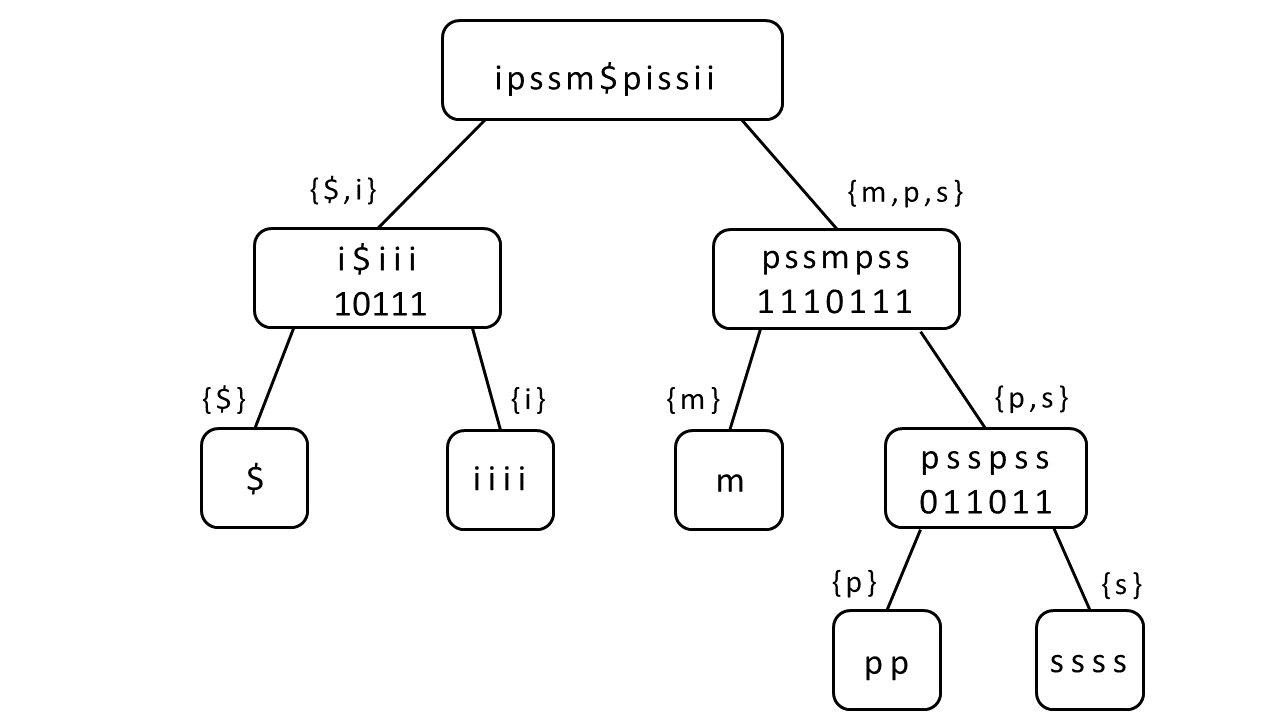
\includegraphics[width=\columnwidth]{waveletTree.png}
			\caption{Stablo valića za navedeni primjer}
			\label{fig:waveletTree}
		\end{center}
	\end{figure}

\subsubsection{Konstrukcija polja najduljih zajedničkih prefiksa}

\begin{enumerate}
	\item Polje najduljih zajedničkih prefiksa gradi se prema Algoritmima 1 i 2 iz rada \cite{beller2013} u nekoliko koraka:

	\begin{enumerate}
		\item Vrijednosti polja LCP postavljaju se na nevažeće($\perp$), osim za $LCP[1]$ i $LCP[n+1]$, koji se postavljaju na $-1$. U red $Q$ se stavlja početni interval $I = [i..j] = [1..12]$ i duljina zajedničkog prefiksa $l = 0$:\\
	 	$$LCP = [-1,\perp,\perp,\perp,\perp,\perp,\perp,\perp,\perp,\perp,\perp,\perp,\perp, \perp, -1]$$
		$$Q = [\langle[1..12],0\rangle]$$

		\item c$\omega$-intervali za prvi $\omega$-interval u redu $Q$ izračunavaju se funkcijom $getIntervals$ (Algoritam 1 iz \cite{beller2013}). Za slučaj intervala $\langle[1..12],0\rangle$, koji označava cjelukupni niz i duljinu zajedničkog prefiksa $0$, rješenje su intervali u kojima svi sufiksi (iz sufiksnog polja) počinju istim znakom, a to su:
		$$ [[1..1],[2..5],[6..6],[7..8],[9..12]] $$
što se može i vidjeti iz tablice \ref{tableEx2}.

		\item Za svaki od dobivenih intervala $[lb..rb]$ se potom provjerava vrijednost $LCP[rb+1]$, i ako je ona jednaka $\perp$, u red se  dodaje $\langle[lb..rb],l+1\rangle$, a na indeks $rb+1$ u polju LCP zapisuje se vrijednost $l$. Za prvu iteraciju algoritma, to izgleda ovako:
			\begin{enumerate}
				\item $LCP = [-1,\perp,\perp,\perp,\perp,\perp,\perp,\perp,\perp,\perp,\perp, \perp, -1]$,\\
				$ Q = [\varnothing]$,\\
				$list = [[1..1],[2..5],[6..6],[7..8],[9..12]]$\\
				
				$ [lb..rb] = [1..1]$\\
						
				$LCP[rb+1]=LCP[2]=\perp$\\
				$\rightarrow$ u red dodajemo $\langle[1..1],1\rangle$, i postavljamo $LCP[2]=0$.
				\newline
						
				\item $LCP = [-1,0,\perp,\perp,\perp,\perp,\perp,\perp,\perp,\perp,\perp, \perp, -1]$,\\
			   	$Q = [\langle[1..1],1\rangle]$,\\
			    $list = [[2..5],[6..6],[7..8],[9..12]]$\\
			    
				$[lb .. rb] = [2..5]$\\

				$LCP[rb+1]=LCP[6]=\perp$\\
				$\rightarrow$ u red stavljamo $\langle[2..5],1\rangle$, i postavljamo $LCP[6]=0$.
				\newline
				\item $LCP = [-1,0,\perp,\perp,\perp,0,\perp,\perp,\perp,\perp,\perp, \perp, -1]$,\\
				$Q = [\langle[1..1],1\rangle, \langle[2..5],1\rangle]$,\\
			    $list = [[6..6],[7..8],[9..12]]$\\
				\ldots
			\end{enumerate}

      	\item Ponavljanjem prethodno opisanih koraka konačno se odredi da je vrijednost polja najduljih zajedničkih prefiksa jednaka: 
		$$ LCP = [-1,0,1,1,4,0,0,1,0,2,1,3,-1] $$
	\end{enumerate}
\end{enumerate}


\section{Rezultati}

Prethodno opisani algoritam uspješno je implementiran i ispitan u sklopu ovoga rada, a njegove su performanse uspoređene s originalnom implementacijom autora rada \cite{beller2013} i prošlogodišnjom studentskom implementacijom opisanom u radu \cite{studenti2017}.

Točnost algoritma provjerena je na tri skupine sintetskih podataka različitih veličina abecede -- slučajno generiranim sekvencama DNA i aminokiselina, te na poznatom nasumičnom latinskom tekstu \textit{lorem ipsum}. Duljine ispitnih podataka bile su u rasponu od $20$ do $25000$ ulaznih znakova, a provjera je vršena usporedbom s točnim rješenjima određenima naivnim algoritmom koji radi u kvadratnoj složenosti.

Usporedba performansi vršena je na skupovima sintetskih DNA podataka u rasponu duljina od $100.000$ do $20.000.000$ ulaznih znakova, a vremena izvršavanja i zauzeća memorije određena su korištenjem pomoćnog Linux programa \texttt{time -a \textit{program [argumenti]}}, koji svojim pokretanjem iz naredbene ljuske pokreće i ciljani program, te korištenjem sustavskih poziva prema jezgri mjeri njegove performanse.

Budući da nijedna od postojećih i trenutno javno dostupnih implementacija stabla valića ne podržava operacije potrebne opisanim algoritmima (konkretno algoritmu 1), načinjena je vlastita implementacija istoga, te su svi testovi provedeni koristeći nju. Konstrukcija sufiksnog polja je pak izvršena javno dostupnom bibliotekom \texttt{sais}, točnije njenom C++ varijantom \texttt{saisxx}.

Performanse ovdje opisane implementacije u početnoj izvedbi nisu bile dovoljno dobre, te je stoga izrađena i vlastita izvedba tzv. bitvektora (na kojima se temelji stablo valića), koja je svojom strukturom i operacijama posebno optimizirana za brzo odgovaranje na rang upite, pri tome koristeći kumulativne sume i brze procesorske operacije za brojanje bitova (\texttt{popcount} instrukcije). Nakon te, kao i još nekolicine manjih optimizacija, performanse algoritma značajno su porasle, te se u trenutnom stanju mogu ravnopravno mjeriti čak i s originalnom implementacijom.

Važno je doduše napomenuti da iz nepoznatih razloga čak ni nakon dugotrajnih pokušaja nije bilo moguće na vlastitim računalima na zadovoljavajući način pokrenuti originalnu implementaciju algoritma i izmjeriti njene performanse, jer su dobivani rezultati bili očigledno neispravni, pa su stoga i odbačeni kao takvi. Zato su podaci o trajanju izvršavanja i zauzeću memorije preuzeti i interpolirani iz prošlogodišnjeg rada, uzimajući kao faktore pretvorbe omjere $T_{prosl.impl.}/T_{orig.impl.}$ i $M_{prosl.impl.}/M_{orig.impl.}$. S tim su faktorima potom podijeljena vremena izvršavanja i zauzeća memorije rješenja iz rada \cite{studenti2017}, koja su bila uspješno pokrenuta, i na taj su način dobivene približne vrijednosti performansi implementacije \cite{beller2013}.

Svi izmjereni (i interpolirani) rezultati prikazani su u tablicama \ref{tableTimeComp} i \ref{tableMemComp}, kao i u grafovima \ref{fig:graphTime} i \ref{fig:graphMem}.

\subsection{Usporedba trajanja izvođenja}

Iz prikazanih rezultata trajanja izvođenja na raznim veličinama ulaza vidljivo je da su performanse svih implementacija približno linearne (za istu ulaznu abecedu), što odgovara teoretskoj složenosti algoritma. No također je uočljivo i da se implementacije međusobno značajno razlikuju po stvarnim vremenima izvođenja, i to na način da je prošlogodišnja studentska implementacija po performansama najlošija, dok su originalna i naša implementacija otprilike podjednake, a čak je možda prisutna i mala prednost na strani naše, no moguće je također i da je to samo posljedica nedovoljno precizne interpolacije vrijednosti.

\begin{table}[h!]
	\caption{Rezultati usporedbe vremena izvođenja algoritama}
	\label{tableTimeComp}
	\begin{center}
		\begin{tabular}{rlll}
			\toprule
			Duljina & Prošlogodišnja & Originalna & Naša \\
			ulaza & implementacija & implementacija* & implementacija \\
			{[znak]} & [s] & [s] & [s] \\
			\midrule
			100.000	   	& 	0,04 	&	0,03		&	0,03 \\
			250.000		& 	0,16	&	0,12		&	0,09 \\
			500.000		& 	0,35	&	0,26		&	0,17 \\
			750.000		& 	0,53	&	0,40		&	0,26 \\
			1.000.000	& 	0,72	&	0,54		&	0,36 \\
			2.500.000	& 	1,99	&	1,49		&	1,06 \\
			4.639.675	& 	3,72	&	2,78		&	2,22 \\
			5.000.000	& 	4,1		&	3,06		&	2,46 \\
			7.500.000	& 	6,84	&	5,11		&	4,35 \\
			10.000.000	& 	9,27	&	6,92		&	6,38 \\
			12.500.000	& 	12,23	&	9,13		&	8,67 \\
			15.000.000	& 	14,89	&	11,12		&	10,63 \\
			17.500.000	& 	19,16	&	14,30		&	12,69 \\
			20.000.000	& 	21,6	&	16,13		&	15,2 \\
			\bottomrule
		\end{tabular}\\ ~ \\
		* \textit{Vrijednosti interpolirane na temelju rezultata prošlogodišnjeg rada}
	\end{center}
\end{table}

\begin{figure}[h!]
	\begin{center}
		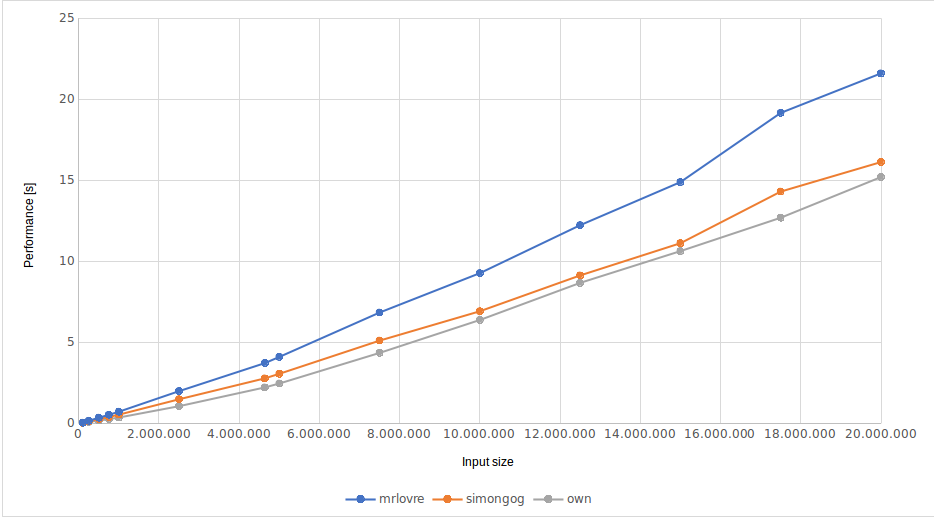
\includegraphics[width=\columnwidth]{timeGraph.png}
 		\caption{Grafički prikaz usporedbe vremena izvođenja različitih implementacija algoritama, prema podacima iz tablice \ref{tableTimeComp}.}
 		\label{fig:graphTime}
	\end{center}
\end{figure}


\clearpage
\subsection{Usporedba zauzeća memorije}

Rezultati mjerenja zauzeća memorije pojedinih implementacija, prikazani u tablici \ref{tableMemComp}, ukazuju na to da prošlogodišnje rješenje za svoj rad zahtjeva značajno više memorije od ostala dva -- otprilike 3 puta više od naše implementacije, i čak 4 puta više od originalne, a razlog tome najvjerojatnije je nekonzervativna uporaba memorije u implementaciji stabla valića koja se u tom rješenju koristi. Naša implementacija, kao što je iz prikazanih podataka vidljivo, nema pati od takvih nedostataka, pa su i njene performanse mnogo bliže onima iz originalnog rada, iako ih još ne uspijeva sasvim dostići.

\begin{table}[h!]
	\caption{Rezultati usporedbe vremena izvođenja algoritama}
	\label{tableMemComp}
	\begin{center}
		\begin{tabular}{rlll}
			\toprule
			Duljina & Prošlogodišnja & Originalna & Naša \\
			ulaza & implementacija & implementacija* & implementacija \\
			{[znak]} & [MB] & [MB] & [MB] \\
			\midrule
			100.000     &   7,32    &   1,83    &   4,328   \\
			250.000     &   12,428  &   3,107   &   5,908   \\
			500.000     &   21,388  &   5,347   &   8,56    \\
			750.000     &   31,592  &   7,898   &   11,92   \\
			1.000.000   &   40,024  &   10,006  &   14,656  \\
			2.500.000   &   97,68   &   24,42   &   32,304  \\
			4.639.675   &   174,224 &   43,556  &   52,372  \\
			5.000.000   &   195,212 &   48,803  &   61,772  \\
			7.500.000   &   277,296 &   69,324  &   88,064  \\
			10.000.000  &   377,372 &   94,343  &   120,644 \\
			12.500.000  &   465,616 &   116,404 &   151,74  \\
			15.000.000  &   553,476 &   138,369 &   181,98  \\
			17.500.000  &   664,256 &   166,064 &   210,7   \\
			20.000.000  &   758,572 &   189,643 &   238,004 \\
			\bottomrule
		\end{tabular}\\ ~ \\
		* \textit{Vrijednosti interpolirane na temelju rezultata prošlogodišnjeg rada}
	\end{center}
\end{table}

\begin{figure}[h!]
	\begin{center}
		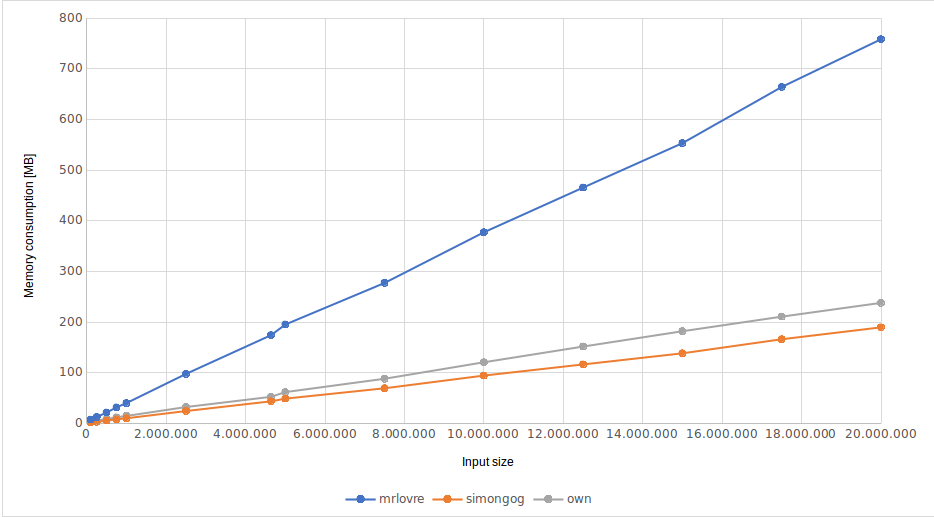
\includegraphics[width=\columnwidth]{memoryGraph.png}
 		\caption{Grafički prikaz usporedbe memorijskog zauzeća različitih implementacija algoritama, prema podacima iz tablice \ref{tableMemComp}.}
 		\label{fig:graphMem}
	\end{center}
\end{figure}

\clearpage
\section{Zaključak}

Rezultati ovog studentskog rada -- implementacija dvaju algoritama opisanih u radu \cite{beller2013} koji se koriste za izračun polja najvećih zajedničkih prefiksa -- pokazali su se uspješnima, jer je ostvarena implementacija, uz ispravan rad, također pokazala i odlične performanse, koje su po memorijskom zauzeću bile tek neznatno lošije od originalne implementacije, a po vremenu izvršavanja potencijalno čak i za nijansu bolje. U tome su pripomogle i brojne optimizacije, od kojih prvenstveno valja izdvojiti vlastitu implementaciju stabla valića temeljenu na optimiziranim bitvektorima, koji za ubrzavanje upita koriste kumulativne sume i ugrađene procesorske instrukcije brojanja bitova.

Implementirani algoritmi, koji u teoriji omogućuju konstrukciju polja najduljih zajedničkih prefiksa u složenosti $O(n \log \sigma)$, i u praksi su pokazali da im je vremenska, ali i memorijska složenost, uz konstantnu veličinu abecede linearna u ovisnosti o duljini ulaznog niza. Također, vrlo dobre performanse algoritama pokazale su da je i njihova primjena u rješavanju praktičnih problema moguća i vrlo obećavajuća.

Daljnji napredak u postizanju još boljih performansi mogao bi se ostvariti na barem dvije razine -- prvo, nadogradnjom implementacije stabla valića iz običnog balansiranog u Huffmanovo ili neko slično, kao i pretvaranjem korištenih bitvektora u RRR strukture, čime bi se u oba slučaja mogla dodatno smanjiti potrošnja memorije; i drugo, analizom vremenski kritičnih operacija te redosljeda pristupa memoriji optimizirati korištenje priručne memorije i dostupnih posebnih instrukcija procesora. Također, daljni rad i analiza samih algoritama također bi mogli dovesti do otkrića nekog novog poboljšanja ili pojednostavnjenja, i time dodatno doprinijeti već i sada vrlo dobrim vremenskim i memorijskim performansama.


\bibliography{literatura}
\bibliographystyle{fer}

\end{document}